\section{The interacting Bose gas}

It is well known that an ideal (non-interacting) Bose gas can undergo a phase-transition into a condensed state where the ground state is macroscopically occupied. If the dimensionality of the system is \emph{$d$}, and the single-particle excitation energy is
\begin{equation}
	\ep_k = \alpha k^\nu,
\end{equation}
then Bose-Einstein condensation (BEC) can take place if $d/\nu > 1$. \todo{Vanskelig å tyde tallet i notatene. Skal det være 1?}
Here, $k$ is a wavenumber. If the total number of particles in the system is $N$, the number of particles in the condensate is $N_0$, and the number of excited states is $N_{>0}$, then 
\begin{equation}
	N = N_0 +N_{>0},
\end{equation}
or equivalently
\begin{equation}
	\frac{N_0}{N} = 1 - \frac{N_{>0}}{N}.
\end{equation}
The Hamiltonian of such a non-interacting system is
\begin{equation}
	\Ha = \sum_{k}\ep_k a_{k}^{\dg}a_{k},
\end{equation}
where the $a^{\dg}$'s create bosons with quantum number  $k$, while the $a$'s correspondingly destroy the same. We take $\ep_k$ to be minimum at $k=0$ (e.g $\ep_k = \frac{\hbar^2k^2}{2m}$, where $m$ is the mass of the particles).
The ground state energy is 
\begin{align}
	E_0 &= \ep_0\ev*{a_{0}^{\dg}a_{0}} = \ep_0\ev*{\hat{N}_{0}} \\
	\hat{N}_{0} &= a_{0}^{\dg}a_{0}
\end{align}
Eigenvalue of $	\hat{N}_{0}$: $N_0 = \#$  particles in condensate
\begin{equation}
	N_0 = \ev*{a_{0}^{\dg}a_{0}}.
\end{equation}
Now, we set $\ev*{a_0^{\dg}} = \ev*{a_0} = \sqrt{N_0}$ which expresses the fact that particles condense in the ground state. 
\begin{align}
	\hat{N} &= \hat{N}_0 + \sum_{k\ne0}a_{k}^{\dg}a_{k} \\
	N&= N_0 + \sum_{k\ne0}\ev*{a_{k}^{\dg}a_{k}} \nonumber \\
	&= N_0 + \sum_{k\ne0}\frac{1}{\e^{\beta\ep_k}-1}
\end{align}
which is an equation for $N_0$ as a function of $T$.
How does all of this change when interactions among bosons is introduced?
We now write the Hamiltonian 
\begin{equation}
	\Ha = \sum_{k}\ep_k a_{k}^{\dg}a_{k} + \sum_{k_1, \dots, k_4}U_{k_1, \dots, k_4}a_{k_1}^{\dg}a_{k_2}^{\dg}a_{k_3}a_{k_4} \delta_{k_1 +k_2, k_3 + k_4}.
\end{equation}
Let us consider weakly interacting Bose gases of alkali atoms $\mathrm{Li, Na, Rb}\dots$.
The interactions are typically van der Waals forces $V(r) \sim \frac{1}{r^6}$. We will model these interactions as contact interactions, i.e. 
\begin{equation}
	U_{k_1, \dots, k_4} = \frac{U}{2V} = \mathrm{constant}.
\end{equation}
(i.e. $\Ha$ is the analog of a Bose-Hubbard model). $V = $ volume. 
\begin{equation}
	\Ha = \sum_{k}\ep_k a_{k}^{\dg}a_{k} + \frac{U}{2V}\sum_{k_1, \dots, k_4}a_{k_1}^{\dg}a_{k_2}^{\dg}a_{k_3}a_{k_4} \delta_{k_1 +k_2, k_3 + k_4}.
\end{equation}
We now consider a condensed state, where we specifically assume
\begin{align}
	N &= N_0 + N_{>0} \\
	N_0 &\gg N_{>0} \\
	N_{0} &\gg 1.
\end{align}
Thus (for later use), we have
\begin{equation}
	\label{eq:Nsquared}
	N^2= (N_0 + N_{>0})^2 \simeq N_0^2 + 2N_0N_{>0}.
\end{equation}
We now set $a_0 = \ev*{a_0} = \sqrt{N_0}$ etc, and expand $\Ha$ to quadratic order in $a_k$, with $k\ne0$, neglecting cubic and quartic terms. Furthermore, we set $\ep_0 = 0$. 
\emph{Kinetic term:}
\begin{equation}
	\sum_{k}\ep_k a_{k}^{\dg}a_{k} = \sum_{k\ne0}\ep_k a_{k}^{\dg}a_{k}.
\end{equation}
\emph{Interaction term:}
\begin{equation}
	\begin{aligned}
	&\frac{U}{2V}\sum_{k_1, \dots, k_4}a_{k_1}^{\dg}a_{k_2}^{\dg}a_{k_3}a_{k_4} \delta_{k_1 +k_2, k_3 + k_4} \\
	&= \frac{U}{2V}N_0^2 + \parbox{5cm}{terms where \emph{at least one} $k_i\ne0$.}
	\end{aligned}
\end{equation}
\begin{itemize}
	\item Consider now first the case where one $k_i\ne0$, i.e. three $k_i = 0$. We then see that $ \delta_{k_1 +k_2, k_3 + k_4} = 0 $.
	Thus, there are \emph{no} terms \emph{linear} in $a_k$ or $a_{k}^{\dg}$, with $k\ne0$. 
	\item Consider next the case where two $k_i$'s $\ne0$, i.e. two $k_i$'s $=0$. 
	There are 6 possibilities: $\binom{4}{2} = 6$. We need to pick 2 $k_i$'s out of the 4 $k_1, k_2, k_3, k_4$. 
\end{itemize}
\begin{align*}
	(k_1, k_2) = 0, && (k_3, k_4)\ne 0 &&\implies a_{k_3}a_{-k_3} \\
	(k_1, k_3) = 0, && (k_2, k_4)\ne 0 &&\implies a_{k_2}^{\dg}a_{k_2} \\
	(k_1, k_4) = 0, && (k_3, k_2)\ne 0 &&\implies a_{k_2}^{\dg}a_{k_2} \\
	(k_2, k_3) = 0, && (k_1, k_4)\ne 0 &&\implies a_{k_1}^{\dg}a_{k_1} \\
	(k_2, k_4) = 0, && (k_1, k_3)\ne 0 &&\implies a_{k_1}^{\dg}a_{k_1} \\
	(k_3, k_4) = 0, && (k_1, k_2)\ne 0 &&\implies a_{k_1}^{\dg}a_{-k_1}^{\dg} \\
\end{align*}
To quadratic order in $a_k, a_k^{\dg}$, the interaction term then becomes
\begin{equation}
	\frac{U}{2V}N_04\sum_{k\ne0}a_{k}^{\dg}a_{k} + \frac{U}{2V}N_0\sum_{k\ne0}\left (a_{k}^{\dg}a_{-k}^{\dg} + a_{k}a_{-k}\right ).
\end{equation}
Hence, we obtain for $\Ha (\ep_0 = 0)$
\begin{equation}
	\begin{aligned}
		\Ha &=\frac{U}{2V}N_0^2 + \sum_{k\ne0}\left (\ep_k + \frac{2U}{V}\right )a_{k}^{\dg}a_{k} \\
		&+ \frac{U}{2V}N_0 \sum_{k\ne0}\left (a_{k}^{\dg}a_{-k}^{\dg} + a_{k}a_{-k}\right )
	\end{aligned}
\end{equation}

An important point to note now, is that at this stage, $\Ha$ is expressed in terms of $\hat{N}_0$, not $\hat{N}$. This is a bit inconvenient, \emph{since $N_0$ is an unknown quantity, while it is $N$ that we prescribe}, and which is therefore known. It therefore behooves us to re-express $\Ha$ in terms of $N$ rather than $N_0$. We proceed as follows:
\begin{align*}
	\Ha &= \frac{U}{2V}N_{0}^{2} + \frac{U}{2V}2N_{0}\sum_{k\ne0}a_{k}^{\dg}a_{k} \\ 
	&+ \sum_{k\ne0}\left (\ep_k + \frac{U}{V}N_0\right )a_{k}^{\dg}a_{k} \\
	&+  \frac{U}{2V}N_0 \sum_{k\ne0}\left (a_{k}^{\dg}a_{-k}^{\dg} + a_{k}a_{-k}\right )
\end{align*}
In the first line: (use \cref{eq:Nsquared})
\begin{equation}
	\frac{U}{2V}(N_0^2 + 2N_0N_{>0}) \simeq \frac{U}{2V}N^2.
\end{equation}
In all other terms, we replace $N_0$ with $N$, to the approximation we are computing: 
\begin{equation}
	\begin{aligned}
		N_0N_{>0} &= (N-N_{>0})N_{>0} \\
		&= NN_{>0} - N_{>0}^2 \\
		&\simeq NN_{>0}.
	\end{aligned}
\end{equation}
Furthermore, using $\ep_k = \ep_{-k}$, we symmetrize the term
\begin{equation}
	\sum_{k\ne0}\left (\ep_k + \frac{U}{V}N\right )a_{k}^{\dg}a_{k} = \frac{1}{2}\sum_{k\ne0}\left (\ep_k + \frac{U}{V}N\right )\left (a_{k}^{\dg}a_{k} + a_{-k}^{\dg}a_{-k}\right )
\end{equation}
Finally, we therefore have the following form for the Hamiltonian
\begin{equation}
	\begin{aligned}
		\Ha &= \frac{U}{2V}N^2 + \frac{1}{2}\sum_{k\ne0}\left (\ep_k + \frac{U}{V}N\right )\left (a_{k}^{\dg}a_{k} + a_{-k}^{\dg}a_{-k}\right ) \\
		&+\frac{U}{2V}N \sum_{k\ne0}\left (a_{k}^{\dg}a_{-k}^{\dg} + a_{k}a_{-k}\right )
	\end{aligned}
\end{equation}
We will now diagonalize this Hamiltonian proceeding more or less along the same lines as we did for the antiferromagnet, or the anisotropic antiferromagnet. 
Introduce new boson operators as follows
\begin{equation}
	\begin{aligned}
		a_k &= u_kA_k-v_kA_{-k}^{\dg} \\
		a_k^{\dg} &= u_kA_k^{\dg}-v_kA_{-k}
	\end{aligned}
\end{equation}
\begin{equation}
	\label{eq:bose_hubbard_hamiltonian_mft}
	\Ha = \frac{U}{2V}N^2 + \frac{1}{2}\sum_{k\ne0}\ep_1\left (a_{k}^{\dg}a_{k} + a_{-k}^{\dg}a_{-k}\right ) + \frac{1}{2}\sum_{k\ne0}\ep_{2}\left ((a_{k}^{\dg}a_{-k}^{\dg} + a_{k}a_{-k}\right )
\end{equation}
\begin{equation}
	\begin{rcases}
		\ep_1 \equiv \ep_k + Un \\
		\ep_2 \equiv Un
	\end{rcases}
	n = \frac{N}{V}
\end{equation}
Note the constant shift of the energy $\ep_k$, which is a mean-field way of accounting for interactions in the problem. 
Consider the $k$-dependent terms $k$ by $k$:
\begin{equation}
	\begin{aligned}
		a_{k}^{\dg}a_{k} &= \left (u_kA_k^{\dg}-v_kA_{-k}\right )\left (u_kA_k-v_kA_{-k}^{\dg}\right ) \\
		&= u_k^2A_{k}^{\dg}A_{k} + v_{k}^2 A_{-k}A_{-k}^{\dg} \\
		& - v_ku_k\left (A_{k}A_{-k} + A_{k}^{\dg}A_{-k}^{\dg}\right )
	\end{aligned}
\end{equation}
Thus, 
\begin{equation}
	\begin{aligned}
		a_{k}^{\dg}a_{k} + a_{-k}^{\dg}a_{-k} &= u_k^2\left (A_{k}^{\dg}A_{k} +A_{-k}^{\dg}A_{-k}\right ) \\
		& + v_{k}^2\left (A_{-k}A_{-k}^{\dg} + A_{k}A_{k}^{\dg}\right ) \\
		&-2v_ku_k\left (A_{k}^{\dg}A_{-k}^{\dg}+A_{k}A_{-k}\right ).
	\end{aligned}
\end{equation}
\begin{equation}
	\begin{aligned}
		a_{k}^{\dg}a_{-k}^{\dg} &= \left (u_kA_k^{\dg}-v_kA_{-k}\right )\left (u_kA_{-k}-v_kA_{k}^{\dg}\right ) \\
		&= u_k^2A_{k}^{\dg}A_{-k}^{\dg} + v_{k}^2 A_{k}A_{-k} \\
		& - v_ku_k\left (A_{k}^{\dg}A_{k} + A_{-k}A_{-k}^{\dg}\right )
	\end{aligned}
\end{equation}
\begin{equation}
	\begin{aligned}
		a_{k}a_{-k} &= v_k^2A_{-k}^{\dg}A_{k}^{\dg} + u_{k}^2 A_{-k}A_{k} \\
		& - v_ku_k\left (A_{k}^{\dg}A_{k} + A_{-k}A_{-k}^{\dg}\right )
	\end{aligned}
\end{equation}
\begin{equation}
	\begin{aligned}
			a_{k}^{\dg}a_{-k}^{\dg} + a_{k}a_{-k} &= u_{k}^2\left (A_{k}^{\dg}A_{-k}^{\dg} + A_{-k}A_{k}\right ) \\
			&+ v_k^2\left (A_{k}A_{-k} + A_{-k}^{\dg}A_{k}^{\dg}\right ) \\
			& -2u_kv_k\left (A_{k}^{\dg}A_{k} + A_{-k}A_{-k}^{\dg}\right ).
	\end{aligned}
\end{equation}
Insert in \cref{eq:bose_hubbard_hamiltonian_mft}
\begin{equation}
	\begin{aligned}
	&\ep_1\left (a_{k}^{\dg}a_{k} + a_{-k}^{\dg}a_{-k}\right ) + \ep_{2}\left (a_{k}^{\dg}a_{-k}^{\dg} + a_{k}a_{-k}\right ) \\
	&= \ep_{1}\left [u_k^2\left (A_{k}^{\dg}A_{k} +A_{-k}^{\dg}A_{-k}\right ) + v_{k}^2\left (A_{-k}^{\dg}A_{-k} + A_{k}^{\dg}A_{k}\right ) + 2v_k^2\right . \\
	&\qquad \left .-2v_ku_k\left (A_{k}^{\dg}A_{-k}^{\dg}+A_{k}A_{-k}\right )\right ] \\
	&\quad+ \ep_2 \left [u_{k}^2\left (A_{k}^{\dg}A_{-k}^{\dg} + A_{-k}A_{k}\right )+ v_k^2\left (A_{k}A_{-k} + A_{-k}^{\dg}A_{k}^{\dg}\right )\right . \\
	&\quad \qquad \left . -2u_kv_k\left (A_{k}^{\dg}A_{k} + A_{-k}^{\dg}A_{-k}\right ) - 2u_kv_k\right ]
	\end{aligned}
\end{equation}

\begin{equation}
	\begin{aligned}
		A_{k}^{\dg}A_{k}: && \ep_1(u_k^2 + v_k^2)-2\ep_2 u_kv_k \\	A_{-k}^{\dg}A_{-k}: && \ep_1(u_k^2 + v_k^2)-2\ep_2 u_kv_k \\
		A_{k}^{\dg}A_{-k}^{\dg}: && \ep_2(u_k^2 + v_k^2)-2\ep_1 u_kv_k\\
		A_{k}A_{-k}: && \ep_2(u_k^2 + v_k^2)-2\ep_1 u_kv_k
	\end{aligned}
\end{equation}
Constant terms appearing when commuting $A_{k}A_{k}^{\dg} = 1 + A_{k}^{\dg}A_{k}$:
\begin{equation}
	-2\ep_2u_kv_k + 2v_k^2\ep_1
\end{equation}
\begin{align*}
	u_k^2-v_k^2 = 1 &\rightarrow \begin{cases*}
		u_k = \cosh(\theta) \\
		v_k = \sinh(\theta)
	\end{cases*} \\
	u_k^2 + v_k^2 &= \cosh(2\theta) \\
	2u_kv_k &= \sinh(2\theta)
\end{align*}
We now adjust $\theta$ such that all terms $A_{k}A_{-k}^{\dg}$ and  $A_{k}A_{-k}$ vanish.

\begin{align*}
	\ep_2(u_k^2 + v_k^2) &= \ep_1u_kv_k \\
	u_k^2 &= \frac{1}{2}\left (1 +\frac{\ep_1}{\sqrt{\ep_1^2-\ep_2^2}}\right ) \\
	v_k^2 &= \frac{1}{2}\left (-1 +\frac{\ep_1}{\sqrt{\ep_1^2-\ep_2^2}}\right )  \\
	4u_k^2v_k^2 &= \frac{\ep_2^2}{\ep_1^2-\ep_2^2} \implies
	2u_kv_k = \frac{\ep_2}{\sqrt{\ep_1^2-\ep_2^2}} \\
	u_k^2 + v_k^2 &= \frac{\ep_1}{\sqrt{\ep_1^2-\ep_2^2}}.
\end{align*}
Thus, the coefficients of $A_{k}^{\dg}A_{k}$ and  $A_{-k}^{\dg}A_{-k}$ is thus 
\begin{equation}
	\frac{1}{2}\left [\ep_1(u_k^2 + v_k^2) -\ep_2 2u_kv_k\right ] = \frac{1}{2}\left (\frac{\ep_1^2-\ep_2^2}{\sqrt{\ep_1^2-\ep_2^2}}\right ) = \frac{1}{2}\sqrt{\ep_1^2-\ep_2^2}.
\end{equation}
Thus,
\begin{equation}
	\begin{aligned}
		\Ha &= \frac{U}{2V}N^2 + \frac{1}{2}\sum_{k\ne0}\left (2v_k^2\ep_1 - 2\ep_2 u_kv_k\right ) \\
		&+ \frac{1}{2}\sum_{k\ne0}E_k\left (A_{k}^{\dg}A_{k} + A_{-k}^{\dg}A_{-k}\right )
	\end{aligned}
\end{equation}
with
\begin{equation}
	\begin{aligned}
	E_k &= \sqrt{\ep_1^2-\ep_2^2} = \sqrt{(\ep_k + nU)^2-(nU)^2} \\
	&= \left [\ep_k(\ep_k + 2nU)\right ]^{\frac{1}{2}}
	\end{aligned}
\end{equation}
Note the delicate cancellation of the $(nU)^2$-terms.

When $U=0$, $E_k=\ep_k$. 
When $U=\ne0$, the spectrum changes drastically as $k\rightarrow0$.
While $\ep_k \sim k^2$, 
\begin{equation}
	E_k = \left (\frac{\hbar^2}{2m}2Un\right )^{\frac{1}{2}}k \equiv \hbar ck; \qquad k\rightarrow 0,\, U\ne0 .
\end{equation}
\begin{equation}
	c = \left (\frac{Un}{m}\right )^{\frac{1}{2}}
\end{equation}
may be interpreted as the velocity of a density-wave. Later, we shall see that $c$ corresponds to the maximum velocity associated with superfluid flow in the condensate. This is called the critical superfluid velocity, which is seen to vanish when $U\rightarrow0$. Thus, an ideal Bose-Einstein condensate is not a superfluid. 

\subsection{Landau criterion for superfluidity}
\suggestion{Subsection or section?}

Let us consider a fluid in motion with total momentum $\bm{p}$ with respect to some fixed reference frame. 
Imagine that we insert a small object and drag it through the fluid with some velocity $\bm{v}$ with respect to the same fixed frame. 
\begin{center}
	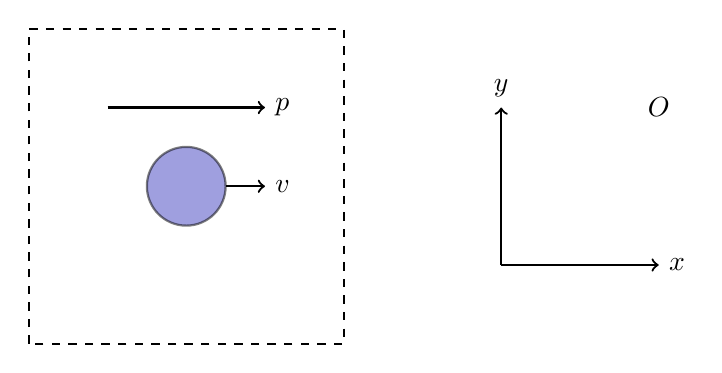
\begin{tikzpicture}
		
		
		\draw[thick, dashed] (0,0) rectangle (4,4);
		\draw[thick, ->] (1, 3) -- (3, 3) node[anchor=west] {$\bm{p}$};
		\draw[thick, ->] (2.5,2) --(3, 2) node[anchor=west] {$\bm{v}$};
		\draw[thick, fill = blue!50!gray,opacity =0.5] (2,2) circle (0.5cm);
		
		%coordinate system
		\draw[thick, ->] (6,1) -- (6,3) node[anchor = south] {$y$};
		\draw[thick, ->] (6, 1) --(8, 1) node[anchor=west] {$x$};
		\node at (8, 3) {$O$};
	\end{tikzpicture}
\end{center}	
Energy of fluid in frame $O$:
\begin{equation}
	E = \frac{p^2}{2M},
\end{equation}
where $M = Nn$, $N$ is the number of particles in fluid element we consider. 
The same energy in the fram of the moving object is 
\begin{equation}
	\begin{aligned}
	E(\bm{v}) &= \frac{1}{2M}\left (\bm{p}-M\bm{v}\right )^2. \\
	&= E - \bm{p}\cdot\bm{v} + \frac{1}{2}Mv^2
	\end{aligned}
\end{equation}
The ground state energy of the fluid in frame $O$:
\begin{equation}
	E_0 = 0.
\end{equation}
The ground state energy of the fluid in the frame of the moving object
\begin{equation}
	E_{\text{GS}}(\bm{v}) = E_0 + \frac{1}{2}Mv^2.
\end{equation}
Imagine now that out of the ground state, we create a single excitation of momentum $\bm{p}$, with energy \emph{$\ep_p$}.
In frame $O$:
\begin{equation}
	E_{\text{ex}} = E_0 + \ep_p.
\end{equation}
But that means that in the frame moving with the obstacle, we have

\begin{align}
	E_{\text{ex}}(\bm{v}) &= E_0 + \ep_p -\bm{p}\cdot \bm{v}  + \frac{1}{2}Mv^2 \\
	\Delta E &= E_{\text{ex}}(\bm{v}) - E_{\text{GS}}(\bm{v}) = \ep_{p}-\bm{p}\cdot\bm{v}.
\end{align}
In other words, dragging an object through the fluid changes the energy required to make an excitation. If $\ep_p - \bm{v}\cdot\bm{p}<0$, the the system \emph{gains} energy by creating excitations, i.e. energy is lowered byu this. This happens at a velocity 
\begin{equation}
	v = \frac{\ep_p}{p}.
\end{equation}
The minimum velocity required, is called the critical velocity, and is given by
\begin{equation}
	v_C = \min\frac{\ep_p}{p}.
\end{equation}
This is the lowest velocity one can drag an obstacle thourgh the fluid and create single-particle excitations, i.e. scattering. Below this velocity, no scattering takes place and the fluid is \emph{superfluid}. For the non-interacting Bose-gas, we have $\ep = \frac{p^2}{2m}$, for which
\begin{equation}
	v_C = \min \frac{p}{2m} =0.
\end{equation}
An ideal Bose gas is not a superfluid. 
With interactions, we found
\begin{align}
	E_p &= \sqrt{\ep_p(\ep_p + Un)} = \sqrt{\frac{Un}{m}}p + \cdots \\
	v_C &= \min\sqrt{\frac{Un}{m}} = \sqrt{\frac{Un}{m}}.  
\end{align}
The interacting Bose gas can  flow with a velocity up to $v_C = \sqrt{\frac{Un}{m}}$ without scattering and therefore exhibits superfluidity. Repulsive interactions are required to stabilize superfluidity. 


\subsection{Condensate fraction}

We have the following relation between the total $\#$ particles in the system, $N$, and the number of particles in the condensate, $N_0$:
\begin{equation}
	N = N_0  + \sum_{k\ne0}\ev*{a_{k}^{\dg}a_{k}}
\end{equation}
Introducing the Bogoliubov operators, we then have
\begin{align}
	N &= N_0 + \sum_{k\ne0}\left [u_k^2\ev*{A_{k}^{\dg}A_{k}} + v_k^2\ev*{A_{-k}A_{-k}^{\dg}}\right ] \nonumber\\
	&= N_0 + \sum_{k\ne0}v_k^2 + \sum_{k\ne0}(u_k^2 + v_k^2)\ev*{A_{k}^{\dg}A_k}\nonumber \\
	&= N_0 + \sum_{k\ne0}v_k^2 + \sum_{k\ne0}\frac{u_k^2 + v_k^2}{\e^{\beta E_k}-1}.
\end{align}
At $T = 0$, the last term gives no contribution, such that we have
\begin{equation}
	N = N_0 + \sum_{k\ne0}v_k^2.
\end{equation}
The condensate fraction may then be expressed as \todo{$\frac{N_0}{N} = 1-\frac{1}{N}\sum_k v_k^2$ ?}
\begin{align}
	\frac{N_0}{N} &= 1-\sum_{k\ne0}v_k^2 \\
	v_k^2 &= \frac{1}{2}\left (-1 + \frac{\ep_1}{\sqrt{\ep_1^2-\ep_2^2}}\right )\\
	\ep_1 &= \ep_k + Un;\quad \ep_2 = Un \nonumber\\
	U\rightarrow 0 &\implies v_k^2 = 0 \implies\nonumber \\
	\frac{N_0}{N} &= 1.
\end{align}
With finite interactions, we get a depletion of the condensate fraction even at $T = 0$. 
Consider now the case $d = 3$.
\begin{align}
	D(\ep) &= K\sqrt{\ep} \\
	\frac{N_0}{N} &= 1- \frac{K}{2}\int_0^{\infty}\dd{\ep}\sqrt{\ep}\left (-1 + \frac{\ep_1}{\sqrt{\ep_1^2-\ep_2^2}}\right ) 
\end{align}
\begin{align}
	\ep &= \ep_1 - Un \nonumber\\
	\ep_1^2-\ep_2^2 &= (\ep_1-\ep_2)(\ep_1 + \ep_2) 
\end{align}
\begin{align}
	\frac{N_0}{N} &= 1- \frac{K}{2}\int_{Un}^{\infty}\dd{x}\sqrt{x-Un}\left (-1 + \frac{x}{\sqrt{x^2-(Un)^2}}\right ) \\
	&= 1-\frac{K}{2}(I_1 - I_2) 
\end{align}
\begin{align}
	I_1 &= \int_{Un}^{\infty}\dd{x}\frac{x}{\sqrt{x + Un}} \\
	I_2 &= \int_{Un}^{\infty}\dd{x} \sqrt{x-Un}.
\end{align}
These integrals will be performed with upper limit $A$, and then let $A\rightarrow\infty$.
\begin{equation}
		I_2 = \frac{2}{3}\left (A-Un\right )^{\frac{2}{3}},
\end{equation}
\begin{equation}
	\begin{aligned}
			I_1 &= \left [\left (\frac{1}{3}\left (x+Un\right )- Un\right )2\sqrt{x+Un}\right ]_{Un}^{A}  \\
		&= \left (\frac{2}{3}\left (A+Un\right )- 2Un\right )\sqrt{A+Un}- \frac{2}{3}Un\cdot 2\sqrt{2Un},
	\end{aligned}
\end{equation}
\begin{equation}
	\lim\limits_{A\rightarrow\infty} (I_1-I_2) = \frac{4}{3}Un\sqrt{2Un}
	= \frac{2}{3}\left (2Un\right )^{\frac{2}{3}}.
\end{equation}
The filling fraction is
\begin{tcolorbox}
\begin{equation}
	\frac{N_0}{N} = 1- \frac{K}{3}\left (2Un\right )^{\frac{3}{2}}.
\end{equation}
\end{tcolorbox}


